% =====================================================================
% Person 3 -- text for Sections 4, 5.3, 6.3 and 7.3 + bibliography entries
% Each block replaces the matching "% TODO (Person 3)" in main.tex.
% Figures needed (same folder as main.tex):
%   fig_5_3_EI_departments.png, fig_5_3_departments_vs_communities.png
% All numbers come from results_RQ3.zip (rq3_summary.json and the tables).
% =====================================================================


% ---------------------------------------------------------------------
% BLOCK 1 -> Section 4 (replace the template text under \section{Validity and Reliability})
% ---------------------------------------------------------------------
%<<SECTION4
\textbf{Validity.} We use e-mail as a proxy for working relationships, and
this proxy has four limits. First, an edge only records that at least one
e-mail was sent, so a single message, such as a reply to an announcement,
counts as much as daily collaboration; some edges are therefore not real
working relationships (errors of commission) \cite{borgatti2018}. Second, the
data only covers e-mails among members of the institution: e-mails with
outsiders, meetings, phone calls and chat are missing (errors of omission).
This is why 19 members (1.9\%) appear as isolated nodes, although they surely
communicate in other ways. Third, the data is anonymised and has no attribute
except the department, so we cannot check members' roles or the period in
which the e-mails were collected. Fourth, we take the department labels as
given: each member belongs to exactly one of 42 departments, even if some
people may work for two units, and 7 departments have fewer than five
members, which makes their measures unstable. The network is therefore a
valid picture of \emph{who} e-mails \emph{whom} inside the institution, but a
weaker picture of how strongly people work together.

\textbf{Reliability.} The study can be repeated exactly. The data is public
(Section~\ref{datasets}) and all group members built the networks with the
same code and rules, published in our GitHub repository. As an independent
check, our whole network has 24{,}929 directed edges after removing
self-loops, the same number of static edges that SNAP reports for the
timestamped version of the dataset. Most measures are deterministic. Every
procedure that uses randomness (random baselines, permutation tests, Louvain,
rewired networks) uses the fixed seed 42, and we report the number of
permutations or random networks next to each result. Because Louvain can give different
communities on different runs, Section~\ref{sec:departments} also reports its
stability over 20 seeds. All measures
were computed in Python with NetworkX 3.7.
%>>SECTION4


% ---------------------------------------------------------------------
% BLOCK 2 -> Section 5.3 (replace "% TODO (Person 3)" under \subsection{Departments as communication boundaries (RQ3)})
% ---------------------------------------------------------------------
%<<SECTION53
To answer RQ3 we look at the department boundary from three sides: whether
members e-mail their own department more than chance (H1--H3), whether the
groups that form from the e-mails match the departments (H4, H5), and whether
e-mails across departments differ from e-mails inside them (H6). Every test
compares the network with a null model in which departments and e-mails are
unrelated (Table~\ref{tab:rq3}).

\textbf{H1: members prefer their own department.} If departments are
boundaries, most e-mails should stay inside them. About one edge in three
(34.7\%) joins two members of the same department, while only one in twenty
(4.7\%) would if e-mails ignored departments. Put differently, two colleagues
from the same department are about eleven times more likely to be connected
than two from different departments. The assortativity coefficient
\cite{newman2003}, which is 0 when people mix at random, confirms this with a
value of 0.31. Because e-mail links are not independent of each other, we
tested the result with the Quadratic Assignment Procedure (QAP)
\cite{krackhardt1988}: it correlates the e-mail matrix with a matrix that marks
same-department pairs, then shuffles the departments 5{,}000 times. No shuffle
came close to the observed correlation, so the preference is significant
($p=0.0002$). The boundary is not closed, however: two thirds of all edges
still cross departments.

\textbf{H2: some departments are much more closed than others.} H1 describes
the institution as a whole, so we next asked \emph{which} departments are
closed. The E--I index \cite{krackhardtstern1988} compares a department's
external and internal edges: it is $-1$ if all edges stay inside and $+1$ if
all go outside. A small department has few colleagues to write to, so
Figure~\ref{fig:ei} shows each department next to the value it would have if
e-mails were random. Of the 35 departments with at least five members, 34 are
significantly more closed than this baseline (adjusted $p<0.05$ after the
Benjamini--Hochberg correction for multiple tests \cite{benjamini1995}). The
differences between them are large. Department~14 is the only one with more
internal than external edges and behaves like a silo; departments~17 and~7 come
close. Departments~6 and~23, instead, are almost as open as random e-mailing,
and many of their members write to no one in their own department. We
considered relating closure to department size, but small departments cannot
have many internal edges, so such a correlation would mainly reflect size.

\textbf{H3: who is outside a department's component.} Section~\ref{sec:structure}
found that many members of departments~21 and~1 are outside the largest
component of their department network. In department~21, 10 of the 15 e-mail only colleagues in other departments, while
5 send no e-mail at all. In department~1, the 9 members are split equally
between small separate groups, contacts outside the department, and no e-mail.
Communication with other departments therefore explains most of the gap in
department~21, but only a third of it in department~1.

\textbf{H4: e-mail groups join departments together.} If departments were the
real units of communication, a method that sees only the e-mails should find
them again. The Louvain method \cite{blondel2008} finds 9 communities (plus the
19 isolated members), with a modularity much higher than in random networks
with the same degrees. The 42 departments, used as groups, reach 70\% of this
modularity: they explain a large part of the community structure, but not all
of it. Figure~\ref{fig:communities} shows why. Each department mostly stays
inside one community (86\% of its members on average), but each community
contains several departments; the largest joins 27 of them, and only one
community (C7) is almost a single department, department~14 again. The informal
groups are thus coarser than the formal ones: they combine departments rather
than cut across them. The agreement measures show a moderate match (NMI 0.60,
ARI 0.36 \cite{danon2005,hubert1985}), which hardly changes over 20 seeds; even
at a resolution that yields 42 communities, NMI only rises to 0.73.

\textbf{H5: a few department pairs and one hub department.} To see which
departments end up together, we counted the edges between every pair of
departments. Three quarters of the pairs (641 of 861) exchange some e-mail, but
half of all cross-department edges fall in only 61 pairs. Most of the busiest
pairs, such as departments~4 and~5 or~21 and~22, sit in the same Louvain
community, which explains how the communities form. Department~36 plays a
special role: with 2\% of the members, it takes part in 23\% of all
cross-department edges and writes to 40 of the 41 other departments, like a
service unit for the whole institution (see Section~\ref{sec:centrality}).

\textbf{H6: e-mails across departments are answered less often.} Finally, a
boundary can change the kind of communication, not only its amount. Splitting
the reciprocity of Section~\ref{sec:structure}, 75\% of links inside
departments are answered, against 69\% across departments. The difference is
larger than in all 5{,}000 shuffles ($p=0.0002$): e-mail between departments is
more often one-way.

\begin{table}[ht]
\centering
\small
\begin{tabular}{llrrr}
\toprule
 & Measure & Observed & Null mean & $p$ \\
\midrule
H1 & Share of edges within departments  & 0.347 & 0.047    & 0.0002 \\
H1 & Assortativity by department          & 0.314 & $-0.002$ & 0.0002 \\
H1 & QAP correlation $r$                  & 0.226 & 0.000    & 0.0002 \\
H2 & E--I index, whole network            & 0.329 & 0.907    & 0.0002 \\
H4 & Modularity $Q$, Louvain              & 0.413 & 0.122    & 0.0099 \\
H4 & Modularity $Q$, departments          & 0.288 & $-0.004$ & 0.0099 \\
H4 & NMI, communities vs departments      & 0.596 & 0.062    & 0.0010 \\
H4 & ARI, communities vs departments      & 0.355 & 0.000    & --     \\
H6 & Reciprocity within / between         & 0.752 / 0.689 & --  & 0.0002 \\
\bottomrule
\end{tabular}
\caption{Tests for RQ3. Null models: 5{,}000 permutations of department labels
(H1, H2, H6; for H6 the test is on the difference), 100 degree-preserving
rewired networks ($Q$), 1{,}000 shuffled community assignments (NMI). Louvain: resolution 1, seed 42,
undirected network. One-sided $p$-values; 0.0002 and 0.0099 are the
smallest values these numbers of permutations allow.}
\label{tab:rq3}
\end{table}

\begin{figure}[ht]
\centering
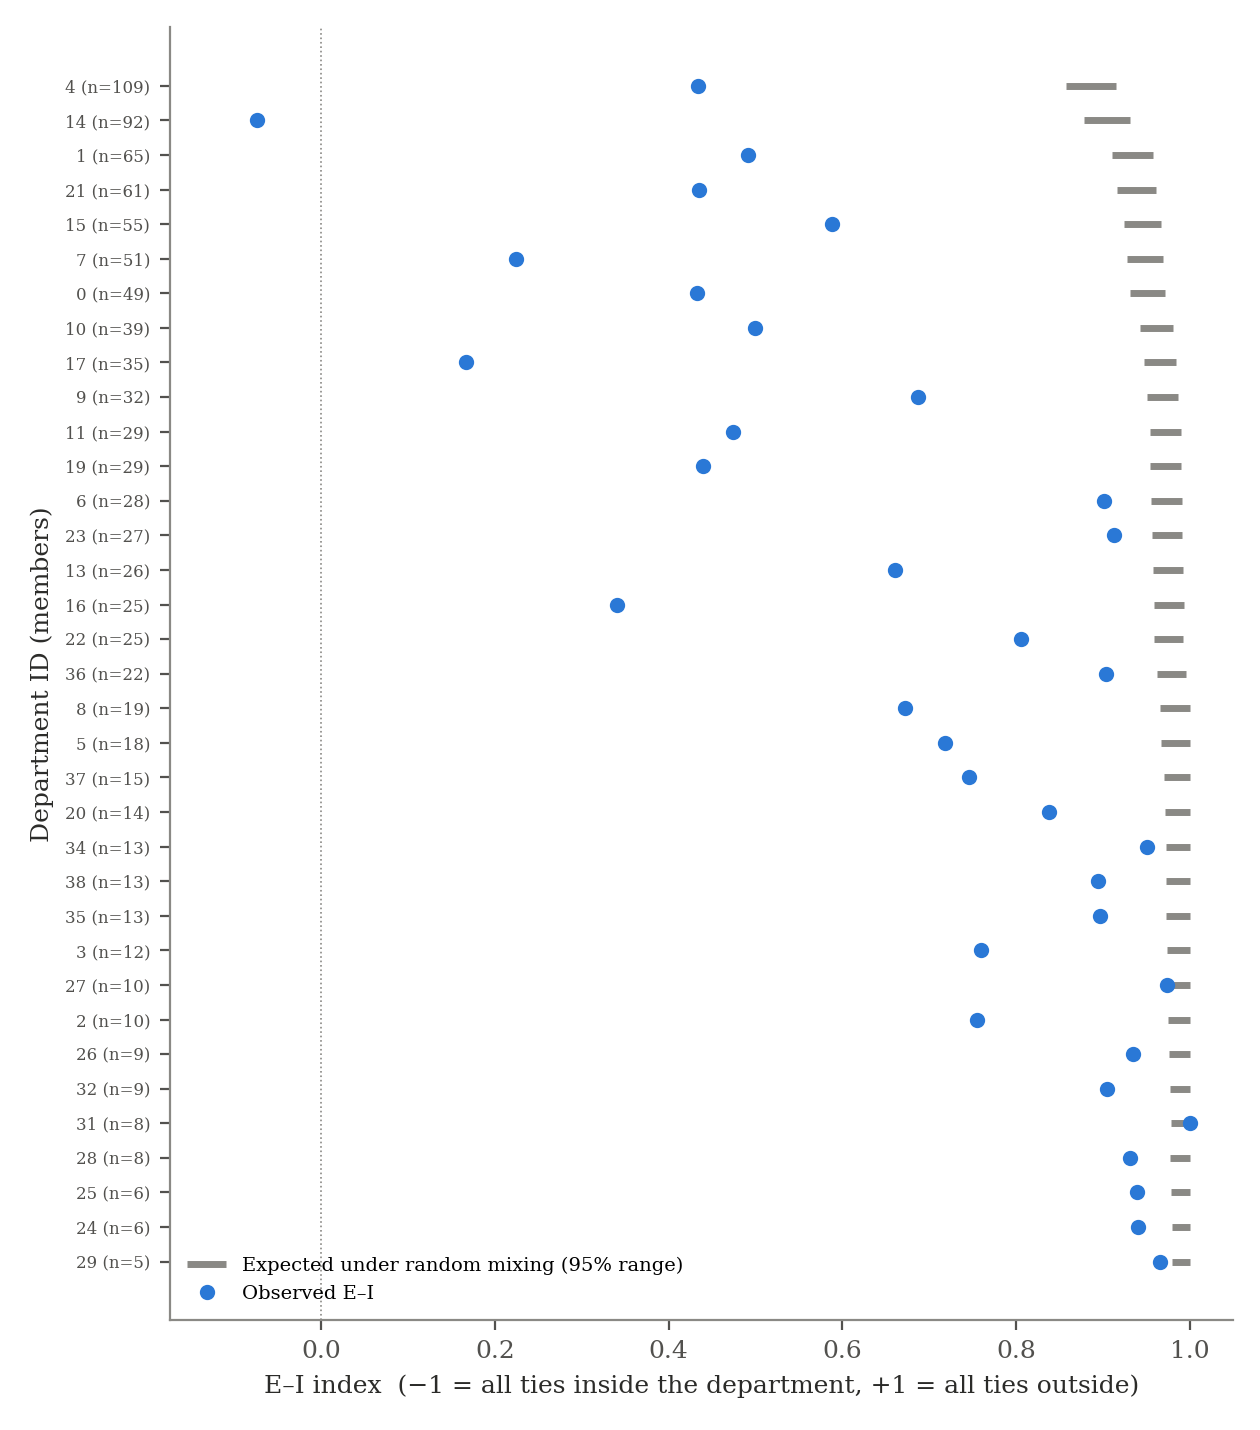
\includegraphics[width=0.72\textwidth]{fig_5_3_EI_departments.png}
\caption{Observed E--I index (dots) of the 35 departments with at least five
members, against the range expected under random mixing (grey, 95\% of
permutations). Dots far to the left of their grey line are departments much
more closed than chance.}
\label{fig:ei}
\end{figure}

\begin{figure}[ht]
\centering
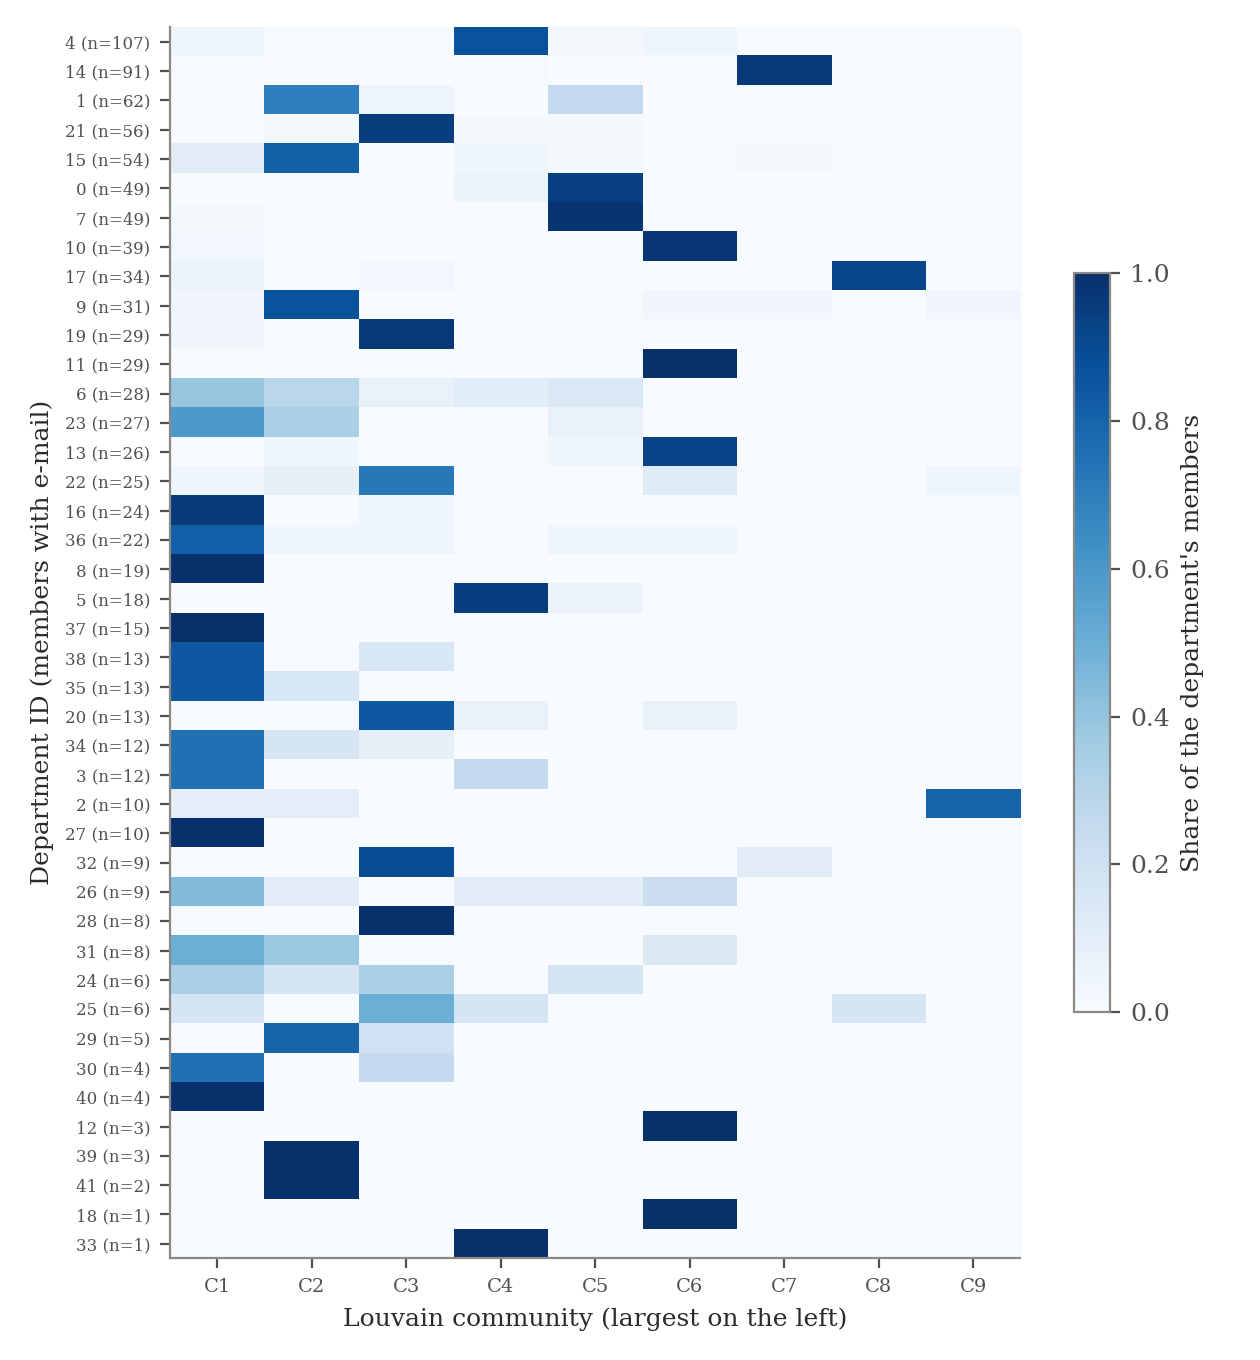
\includegraphics[width=0.72\textwidth]{fig_5_3_departments_vs_communities.png}
\caption{Share of each department's members (rows) in each Louvain community
(columns), isolated members excluded. Most rows have one dark cell (departments
stay together), but many columns have several (communities merge
departments).}
\label{fig:communities}
\end{figure}
%>>SECTION53


% ---------------------------------------------------------------------
% BLOCK 3 -> Section 6.3 (replace "% TODO 6.2 (Person 2), 6.3 (Person 3)": keep Person 2's part)
% ---------------------------------------------------------------------
%<<SECTION63
\subsection{RQ3: departments as boundaries}
Departments are real but permeable boundaries of communication. A member is
about eleven times more likely to e-mail a colleague of the same department,
34 of the 35 tested departments are more closed than chance, and e-mails
inside departments are answered more often. Yet two thirds of the e-mail links
cross departments, and the groups that emerge from the e-mails only partly
match the departments: they keep most departments together but merge them into
a few larger blocks, following the department pairs that e-mail each other
most, while department~36 connects almost all departments. Closure also varies: department~14 works almost as a
silo, while departments~6 and~23 mix almost freely. The formal structure
therefore explains a large part, but not all, of the informal one.
%>>SECTION63


% ---------------------------------------------------------------------
% BLOCK 4 -> Section 7.3 (replace "% TODO 7.2 (Person 2), 7.3 (Person 3)": keep Person 2's part)
% ---------------------------------------------------------------------
%<<SECTION73
\subsection{RQ3: departments as boundaries}
Three limits apply. First, Louvain is randomised and modularity cannot detect
groups below a certain size \cite{fortunato2007}; we measured the effect of
seeds and resolution, but another community method could draw different
groups. Second, many departments are small: their E--I index is uncertain,
seven departments were not tested, and NMI and ARI ignore the 19 isolated
members. Third, QAP shows that sharing a department is associated with
e-mailing, not why: colleagues may also share an office or a project, which
the data does not record. Finally, all results come from a single
institution.
%>>SECTION73


% ---------------------------------------------------------------------
% BLOCK 5 -> bibliography (add before \end{thebibliography})
% ---------------------------------------------------------------------
%<<BIB
\bibitem{benjamini1995} Y.~Benjamini, Y.~Hochberg. Controlling the false
  discovery rate: a practical and powerful approach to multiple testing.
  \emph{Journal of the Royal Statistical Society B}, 57(1):289--300, 1995.
\bibitem{blondel2008} V.~D. Blondel, J.-L. Guillaume, R.~Lambiotte,
  E.~Lefebvre. Fast unfolding of communities in large networks. \emph{Journal
  of Statistical Mechanics}, P10008, 2008.
\bibitem{danon2005} L.~Danon, A.~D\'iaz-Guilera, J.~Duch, A.~Arenas. Comparing
  community structure identification. \emph{Journal of Statistical Mechanics},
  P09008, 2005.
\bibitem{fortunato2007} S.~Fortunato, M.~Barth\'elemy. Resolution limit in
  community detection. \emph{PNAS}, 104(1):36--41, 2007.
\bibitem{hubert1985} L.~Hubert, P.~Arabie. Comparing partitions. \emph{Journal
  of Classification}, 2:193--218, 1985.
\bibitem{krackhardt1988} D.~Krackhardt. Predicting with networks:
  nonparametric multiple regression analysis of dyadic data. \emph{Social
  Networks}, 10(4):359--381, 1988.
\bibitem{krackhardtstern1988} D.~Krackhardt, R.~N. Stern. Informal networks and
  organizational crises: an experimental simulation. \emph{Social Psychology
  Quarterly}, 51(2):123--140, 1988.
\bibitem{newman2003} M.~E.~J. Newman. Mixing patterns in networks.
  \emph{Physical Review E}, 67:026126, 2003.
%>>BIB
